\documentclass[a4paper, 10pt, twoside]{article}
\usepackage[left=2cm, right=2cm, top=2cm, bottom=3cm]{geometry}
\usepackage{amsmath}
\usepackage[shortlabels]{enumitem}
\usepackage{bbold}
\usepackage{cases}
\usepackage{systeme}
\usepackage{graphicx}

\begin{document}

\title{Machine Learning - Theoretical exercise 1}
\author{T\'eo Bouvard}
\maketitle

\section*{Problem 1}
\begin{enumerate}[a)]
    \item According to the sum rule,
          \begin{align*}
              \iint_X \rho(x) \,dx                                                       & = 1                                                   \\
              \int_{-\infty}^{+\infty}\int_{-\infty}^{+\infty} \rho(x_1, x_2) \,dx_1dx_2 & = 1                                                   \\
              \int_{a_2}^{b_2}\int_{a_1}^{b_1} c \,dx_1dx_2                              & = 1 &  & \text{p.d.f is zero outside of these bounds} \\
              c(b_1-a_1)(b_2-a_2)                                                        & = 1                                                   \\
              \frac{1}{(b_1-a_1)(b_2-a_2)}                                               & = c
          \end{align*}

    \item Using the formula to compute the expected value,
          \begin{align*}
              \mathrm{E}(x) & = \int_{-\infty}^{+\infty}\int_{-\infty}^{+\infty} \begin{bmatrix} x_1 \\ x_2 \end{bmatrix}\rho(x_1, x_2) \,dx_1dx_2 \\
                            & = c \int_{a_2}^{b_2}\int_{a_1}^{b_1} \begin{bmatrix} x_1 \\ x_2 \end{bmatrix} \,dx_1dx_2                             \\
                            & = c \int_{a_2}^{b_2} \begin{bmatrix} \frac{b_1^2 - a_1^2}{2} \\ x_2(b_1-a_1) \end{bmatrix} \,dx_2                                                 \\
                            & = c\begin{bmatrix} \frac{b_1^2 - a_1^2}{2}(b_2-a_2) \\ \frac
                  {b_2^2 - a_2^2}{2}(b_1-a_1)\end{bmatrix}
          \end{align*}

          Using $a^2-b^2 = (a-b)(a+b)$, we can factor factor this expression as
          $$\mathrm{E}(x) = c\begin{bmatrix} \frac{(b_1-a_1)(b_1+a_1)(b_2-a_2)}{2} \\ \frac
                  {(b_1-a_1)(b_2+a_2)(b_2-a_2)}{2}\end{bmatrix}$$

          Substituting $c$ with the value computed in the previous question, we can simplify it further as

          \begin{align*}
              \mathrm{E}(x) & = \frac{1}{(b_1-a_1)(b_2-a_2)}\begin{bmatrix} \frac{(b_1-a_1)(b_1+a_1)(b_2-a_2)}{2} \\ \frac{(b_1-a_1)(b_2+a_2)(b_2-a_2)}{2} \end{bmatrix} \\
                            & = \frac{1}{2}\begin{bmatrix} b_1+a_1 \\ b_2+a_2 \end{bmatrix}
          \end{align*}
          
          \begin{align*}
            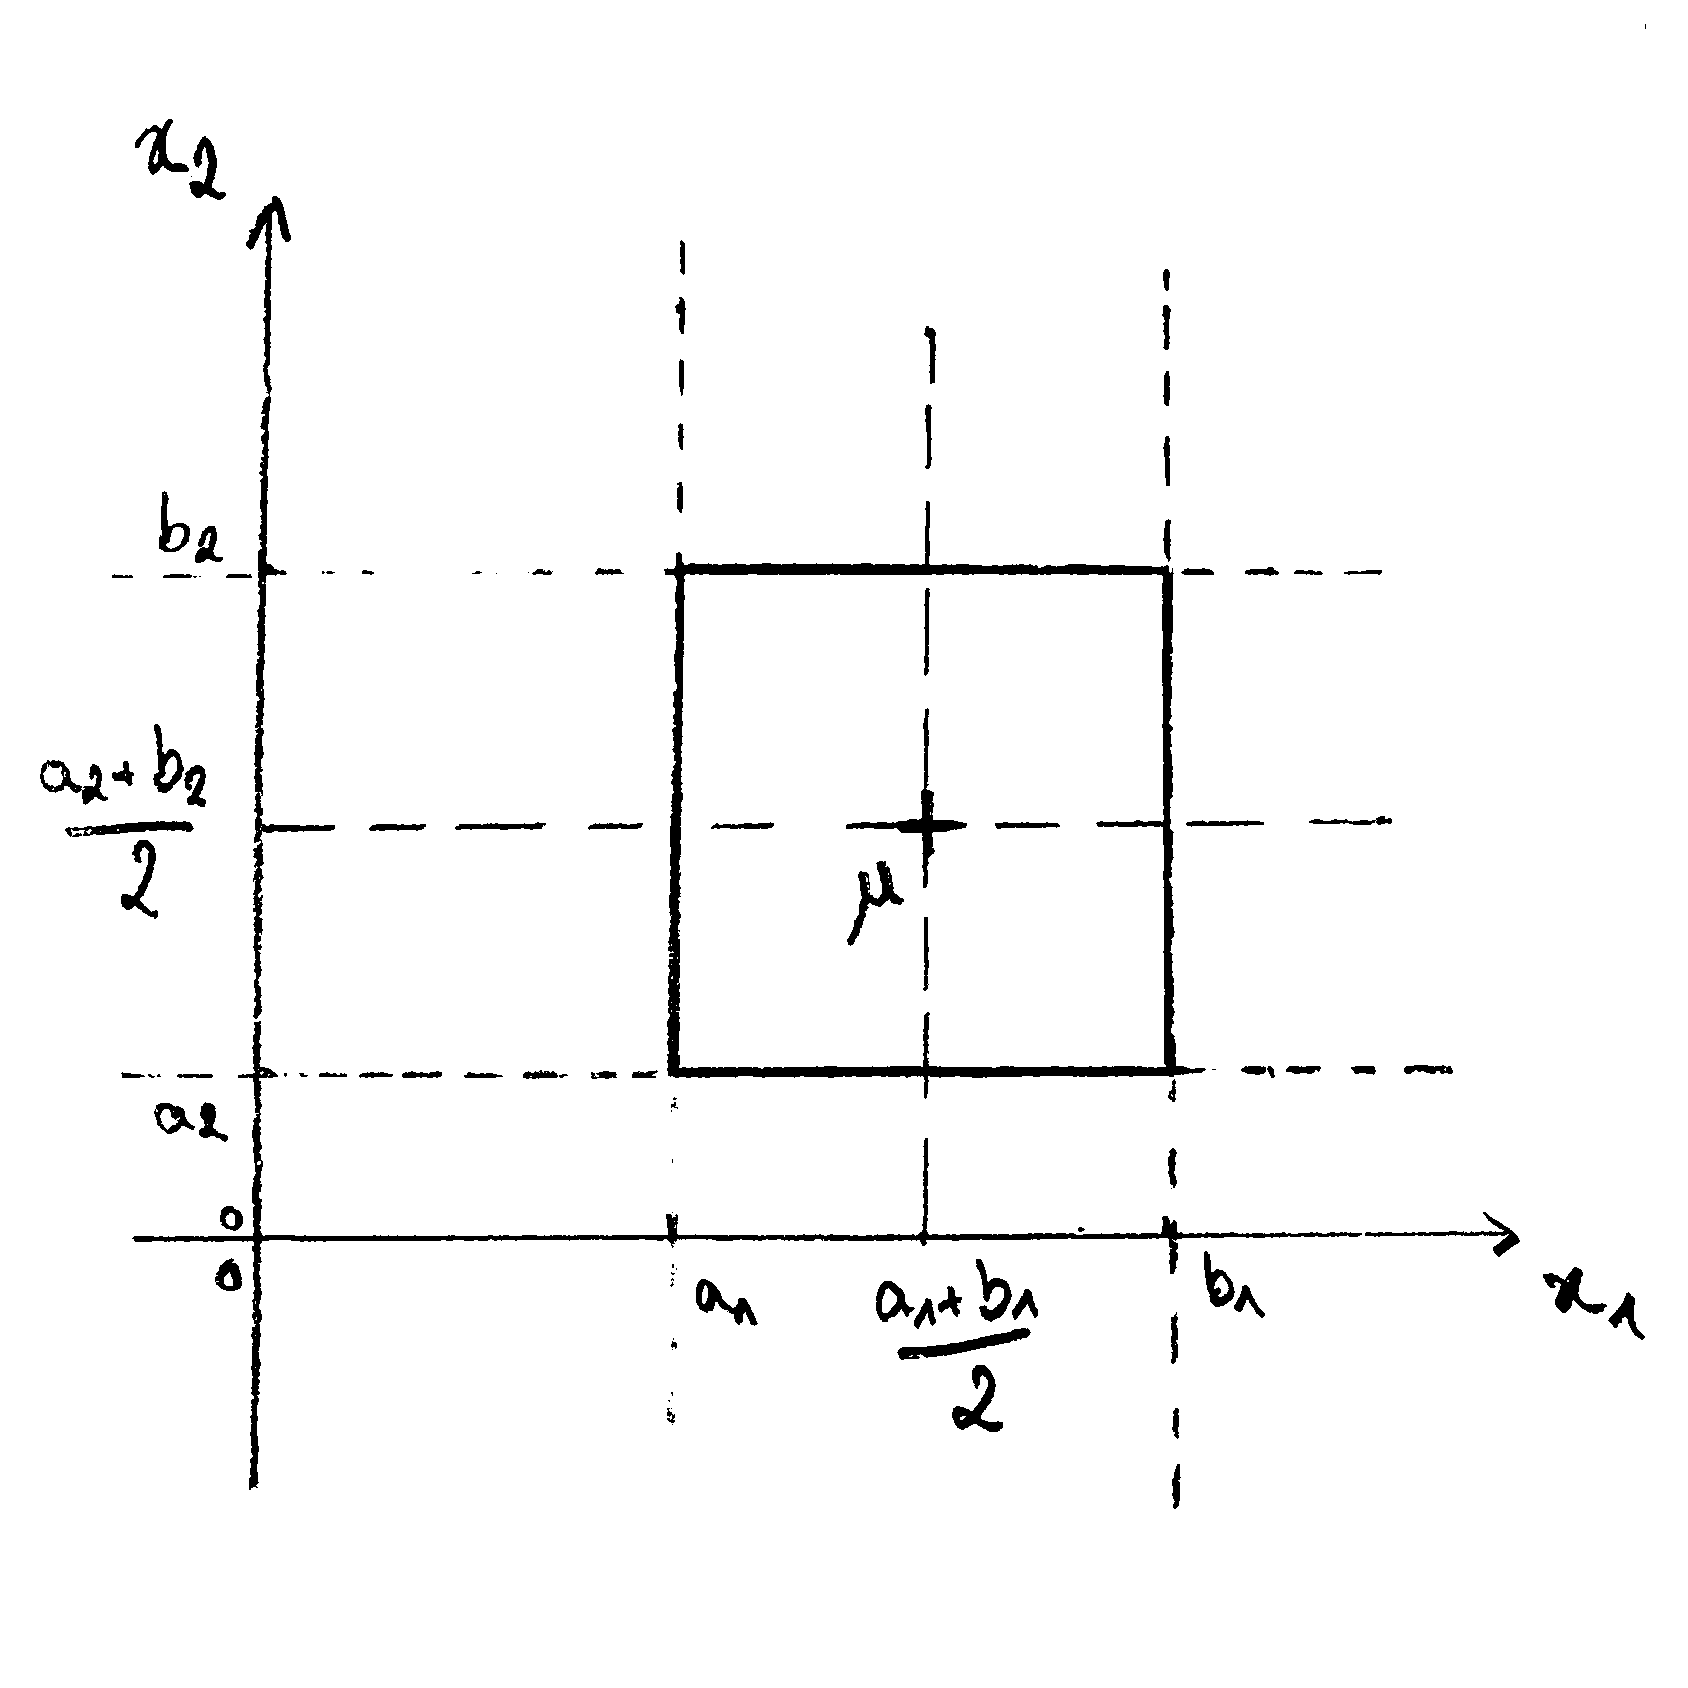
\includegraphics[width=0.5 \textwidth]{sketch1.png}
          \end{align*}


    \item We compute the covariance matrix, defined as follows

          \begin{align*}
              \mathrm{Cov}(x) & = \mathrm{E}((x-\mu)(x-\mu)^T) \\
                              & = \mathrm{E}(xx^T) - \mu\mu^T
          \end{align*}

          Let's compute each term independently.

          \begin{align*}
              \mathrm{E}(xx^T)
               & = \mathrm{E}(\begin{bmatrix} x_1^2 & x_1x_2 \\ x_1x_2 & x_2^2 \end{bmatrix})                                                               \\
               & = \int_{-\infty}^{+\infty}\int_{-\infty}^{+\infty} \begin{bmatrix} x_1^2 & x_1x_2 \\ x_1x_2 & x_2^2 \end{bmatrix}\rho(x_1, x_2) \,dx_1dx_2 \\
               & = c\int_{a_2}^{b_2}\int_{a_1}^{b_1} \begin{bmatrix} x_1^2 & x_1x_2 \\ x_1x_2 & x_2^2 \end{bmatrix}\,dx_1dx_2                               \\
               & = c\int_{a_2}^{b_2} \begin{bmatrix} \frac{b_1^3 - a_1^3}{3} & x_2\frac{b_1^2-a_1^2}{2} \\ x_2\frac{b_1^2-a_1^2}{2} & x_2^2(b_1-a_1) \end{bmatrix}\,dx_2                                                   \\
               & =  c \begin{bmatrix} \frac{b_1^3 - a_1^3}{3}(b_2-a_2) & \frac{b_2^2-a_2^2}{2}\frac{b_1^2-a_1^2}{2} \\ \frac{b_2^2-a_2^2}{2}\frac{b_1^2-a_1^2}{2} & \frac{b_2^3 - a_2^3}{3}(b_1-a_1) \end{bmatrix}                                                                        \\
          \end{align*}

          Substituting $c$ by its value and using $a^3 - b^3 = (a-b)(a^2 + ab + b^2)$,

          \begin{align*}
              \mathrm{E}(xx^T)
               & = \frac{1}{(b_1-a_1)(b_2-a_2)}\begin{bmatrix} \frac{(b_1-a_1)(a_1^2+a_1b_1+b_1^2)(b_2-a_2)}{3} & \frac{(b_2-a_2)(b_2+a_2)(b_1-a_1)(b_1+a_1)}{4} \\ \frac{(b_2-a_2)(b_2+a_2)(b_1-a_1)(b_1+a_1)}{4} & \frac{(b_2-a_2)(a_2^2+a_2b_2+b_2^2)(b_1-a_1)}{3} \end{bmatrix} \\
               & = \begin{bmatrix} \frac{a_1^2+a_1b_1+b_1^2}{3} & \frac{(b_2+a_2)(b_1+a_1)}{4} \\ \frac{(b_2+a_2)(b_1+a_1)}{4} & \frac{a_2^2+a_2b_2+b_2^2}{3} \end{bmatrix}                             \\
          \end{align*}

          And

          \begin{align*}
              \mu\mu^T & = \frac{1}{2}\begin{bmatrix} a_1+b_1 \\ a_2+b_2 \end{bmatrix} \times\frac{1}{2} \begin{bmatrix} a_1+b_1 & a_2+b_2 \end{bmatrix} \\
                       & = \frac{1}{4}\begin{bmatrix} (a_1+b_1)^2 & (a_1+b_1)(a_2+b_2) \\ (a_1+b_1)(a_2+b_2) & (a_2+b_2)^2 \end{bmatrix}
          \end{align*}

          Using the previous results to find the covariance,

          \begin{align*}
              \mathrm{Cov}(x) & = \mathrm{E}(xx^T) - \mu\mu^T                                        \\
                              & = \begin{bmatrix} \frac{a_1^2+a_1b_1+b_1^2}{3} & \frac{(b_2+a_2)(b_1+a_1)}{4} \\ \frac{(b_2+a_2)(b_1+a_1)}{4} & \frac{a_2^2+a_2b_2+b_2^2}{3} \end{bmatrix} - \frac{1}{4}\begin{bmatrix} (a_1+b_1)^2 & (a_1+b_1)(a_2+b_2) \\ (a_1+b_1)(a_2+b_2) & (a_2+b_2)^2 \end{bmatrix} \\
                              & = \frac{1}{12} \begin{bmatrix} 4(a_1^2+a_1b_1+b_1^2) - 3(a_1+b_1)^2 & 3(b_2+a_2)(b_1+a_1)-3(b_2+a_2)(b_1+a_1) \\ 3(b_2+a_2)(b_1+a_1)-3(b_2+a_2)(b_1+a_1) & 4(a_2^2+a_2b_2+b_2^2) - 3(a_2+b_1)^2 \end{bmatrix}                            \\
                              & = \frac{1}{12} \begin{bmatrix} a_1^2-2a_1b_1+b_1^2 & 0 \\ 0 & a_2^2-2a_2b_2+b_2^2 \end{bmatrix}                            \\
                              & = \frac{1}{12} \begin{bmatrix} (a_1-b_1)^2 & 0 \\ 0 & (a_2-b_2)^2 \end{bmatrix}
          \end{align*}

    \item
          $\mathrm{Cov}(x) = \begin{bmatrix}
                  \sigma_{x_1}^2   & \sigma(x_1, x_2) \\
                  \sigma(x_2, x_1) & \sigma_{x_2}^2   \\
              \end{bmatrix}$, so identical elements on the diagonal $\implies \sigma_{x_1} = \sigma_{x_2}$. In other terms, $x_1$ and $x_2$ spread in a similar manner around their respective expected value. \\
          In this problem, having identical elements on the diagonal would mean that $a_1-b_1 = a_2-b_2$, or that the probability density function is a square.
    \item
          $\mathrm{Cov}(x) \text{ diagonal} \implies \sigma(x_1, x_2) = 0 \text{ and } \sigma(x_2, x_1) = 0$, which means that $x_1$ and $x_2$ are uncorrelated.

\end{enumerate}

\section*{Problem 2}

\begin{enumerate}[a)]
    \item We first find the eigenvalues by computing the characteristic equation.

          \begin{align*}
              \det (\Sigma - \lambda I)  & = 0   \\
              \begin{vmatrix} 5 - \lambda & 3 \\ 3 & 5 - \lambda \end{vmatrix} & = 0   \\
              (5-\lambda)^2              & = 3^2 \\
          \end{align*}

          Which implies
          \begin{align*}
               & \begin{cases}
                  5 - \lambda_1 & = -3 \\
                  5 - \lambda_2 & = 3
              \end{cases} \\
               & \begin{cases}
                  \lambda_1 & = 8 \\
                  \lambda_2 & = 2
              \end{cases}
          \end{align*}

          Let $u_1 = \begin{bmatrix}e_{11} \\ e_{21}\end{bmatrix}$ and $u_2 = \begin{bmatrix}e_{12} \\ e_{22}\end{bmatrix}$ be the two eigenvectors of $\Sigma$.

          \begin{align*}
              \Sigma u_1                 & = \lambda_1 u_1 \\
              (\Sigma - \lambda_1 I) u_1 & = 0             \\
              \begin{bmatrix}
                  -3 & 3  \\
                  3  & -3
              \end{bmatrix}
              \begin{bmatrix}
                  e_{11} \\ e_{21}
              \end{bmatrix} & = 0             \\
          \end{align*}
          Which leads to the following system of equations
          \begin{align*}
              \systeme{
                  -3 e_{11} + 3 e_{21} = 0,
                  3 e_{11} - 3 e_{21} = 0
              }
              \implies e_{11} = e_{21}
              \implies u_1 = \frac{1}{\sqrt{2}}\begin{bmatrix}1 \\ 1\end{bmatrix}
          \end{align*}

          We use the same process to find $u_2$.

          \begin{align*}
              \Sigma u_2                 & = \lambda_2 u_2 \\
              (\Sigma - \lambda_2 I) u_2 & = 0             \\
              \begin{bmatrix}
                  3 & 3 \\
                  3 & 3
              \end{bmatrix}
              \begin{bmatrix}
                  e_{12} \\ e_{22}
              \end{bmatrix} & = 0             \\
          \end{align*}
          Which leads to the following system of equations
          \begin{align*}
              \systeme{
                  3 e_{12} + 3 e_{22} = 0,
                  3 e_{12} + 3 e_{22} = 0
              }
              \implies e_{12} = - e_{22}
              \implies u_2 = \frac{1}{\sqrt{2}}\begin{bmatrix}1 \\ -1\end{bmatrix}
          \end{align*}

          Therefore, we have

          \begin{align*}
              \Phi    & = \frac{1}{\sqrt{2}}\begin{bmatrix}1&1\\1&-1\end{bmatrix} \\
              \Lambda & = \begin{bmatrix}8&0\\0&2\end{bmatrix}
          \end{align*}

          We can check our results by verifying that $\Phi \Lambda \Phi^T = \Sigma$.

          \begin{align*}
              \Phi \Lambda \Phi^T & = \frac{1}{\sqrt{2}}\frac{1}{\sqrt{2}}\begin{bmatrix}1&1\\1&-1\end{bmatrix}\begin{bmatrix}8&0\\0&2\end{bmatrix}\begin{bmatrix}1&1\\1&-1\end{bmatrix} \\
                                  & = \frac{1}{2}\begin{bmatrix}8&2\\8&-2\end{bmatrix}\begin{bmatrix}1&1\\1&-1\end{bmatrix}                                                    \\
                                  & = \frac{1}{2}\begin{bmatrix}10&6\\6&10\end{bmatrix}                                                                              \\
                                  & = \begin{bmatrix}5&3\\3&5\end{bmatrix}                                                                                         \\
                                  & = \Sigma
          \end{align*}
          Let $v_1$ and $v_2$ be the principal axes of the probability density function. According to the previous decomposition, we have $v_1 = \sqrt{\lambda_1}u_1$ and $v_2 = \sqrt{\lambda_2}u_2$.
          \begin{align*}
              v_1 & = 2\sqrt{2}\begin{bmatrix}1\\1\end{bmatrix} \\
              v_2 & = \sqrt{2}\begin{bmatrix}1\\-1\end{bmatrix}  \\
          \end{align*}

    \item
    \begin{align*}
        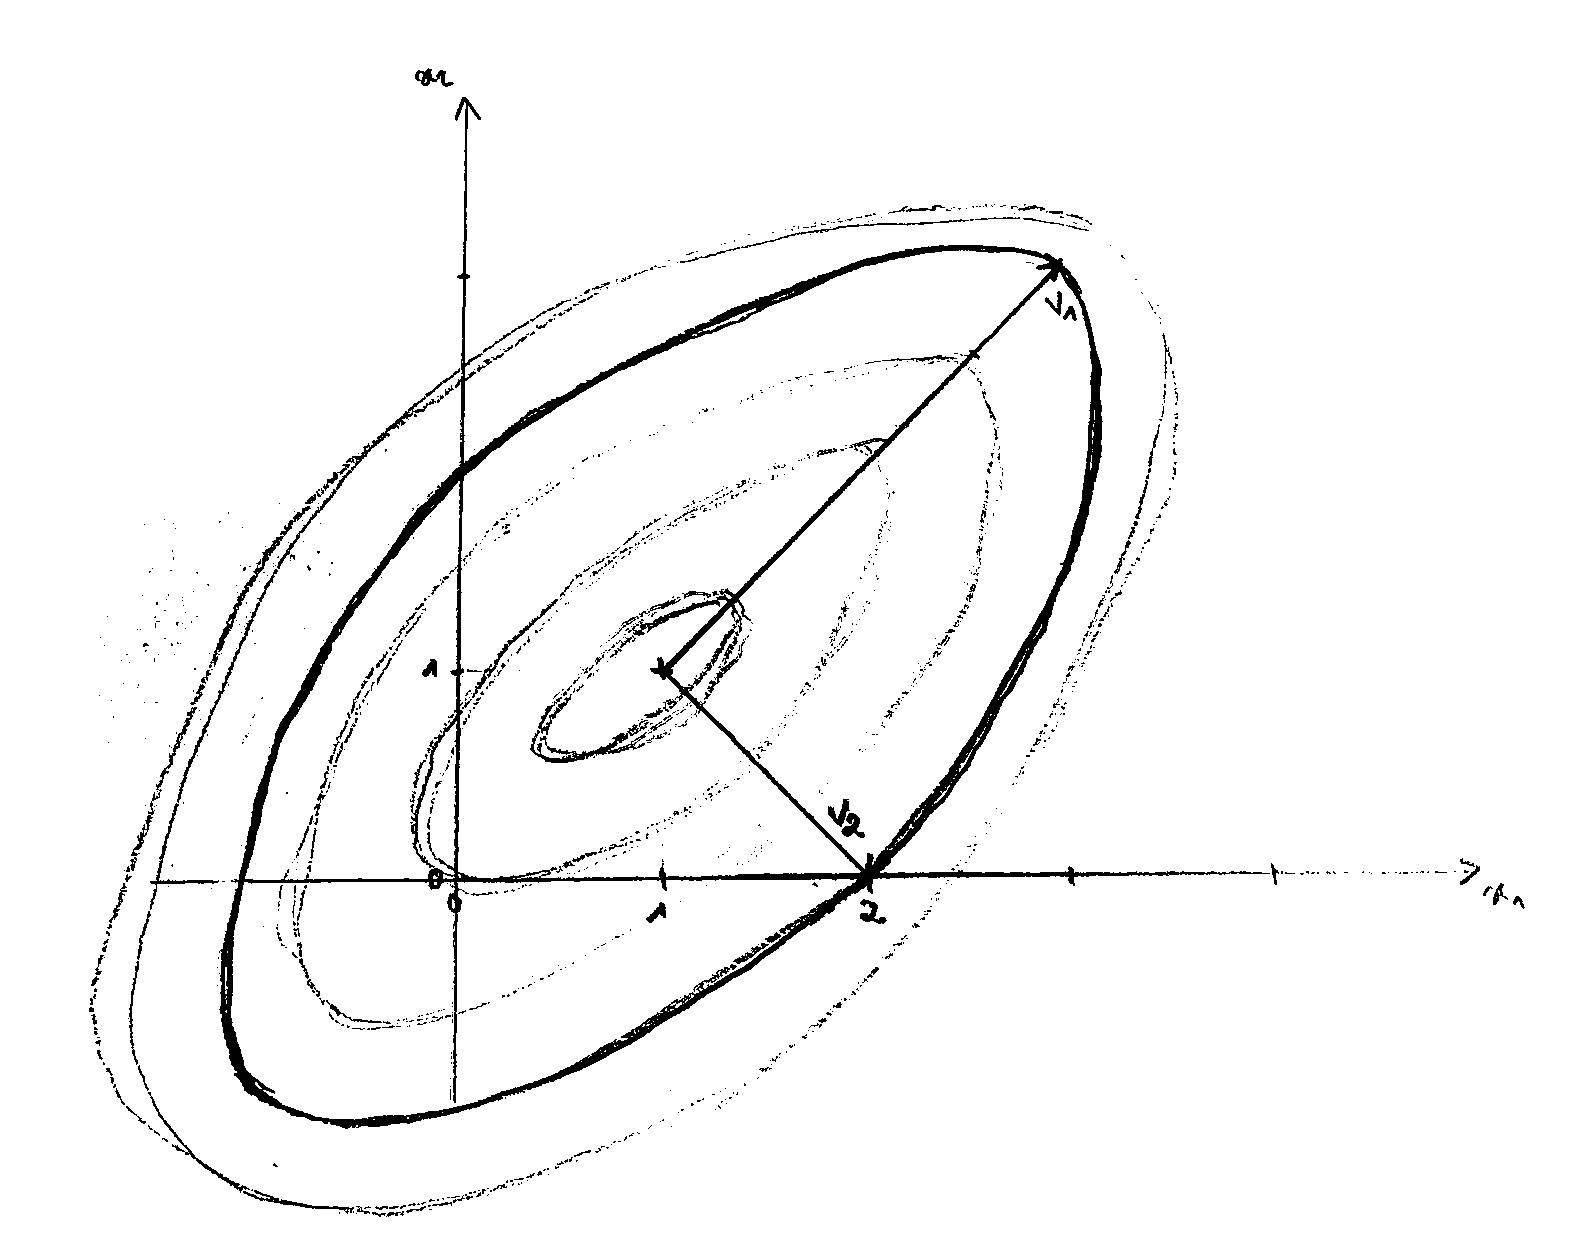
\includegraphics[width=0.7 \textwidth]{sketch2.png}
    \end{align*}

\end{enumerate}


\end{document}
